% % % % % % % % % % % % % % % % % % % % % % % % % % % % % % % % % % % % % % % % % % % %
%                                                                                     %
% Short Sectioned Assignment LaTeX Template Version 1.0 (5/5/12)                      %
% This template has been downloaded from: http://www.LaTeXTemplates.com               %
%                                                                                     %
% Original author:  Frits Wenneker (http://www.howtotex.com)                          %
%                                                                                     %
% Modified by: Fco Javier Sueza Rodríguez (fcosueza@disroot.org)                      %
%                                                                                     %
% Changes:                                                                            %
%	    - Custom Chapters, Sections and Subsections (titlesec package)                %
%           - Document type scrbook (oneside)                                         %
%           - Use babel-lang-spanish package and marvosym                             %
%           - Use hyperref, enumitem, tcolorbox and glossaries packages               %
%           - Use Time New Roman (mathptmx), Helvetic and Courier fonts               %
%                                                                                     %
% License: CC BY-NC-SA 3.0 (http://creativecommons.org/licenses/by-nc-sa/3.0/)        %
%                                                                                     %
% % % % % % % % % % % % % % % % % % % % % % % % % % % % % % % % % % % % % % % % % % % %

%-----------------------------------------------%
%	              Packages                  %
%-----------------------------------------------%

\documentclass[paper=a4, fontsize=11pt, oneside]{scrbook}

% ---- Text Input/Output ----- %

\usepackage[T1]{fontenc}
\usepackage[utf8]{inputenc}
\usepackage{mathptmx}
\usepackage[scaled=.92]{helvet}
\usepackage{courier}
\usepackage[indent=12pt]{parskip}

\usepackage{geometry}
\geometry{verbose,tmargin=3cm,bmargin=3cm,lmargin=2.6cm,rmargin=2.6cm}

% ---- Language ----- %

\usepackage[spanish]{babel}
\usepackage{marvosym}

% ---- Another packages ---- %

\usepackage{amsmath,amsfonts,amsthm}
\usepackage{graphics,graphicx}
\usepackage{titlesec}
\usepackage{fancyhdr}
\usepackage{tcolorbox}
\usepackage{hyperref}
\usepackage{enumitem}
\usepackage[automake]{glossaries}

%--------------------------------------------------------------------%
%                      Customizing Document                          %
%--------------------------------------------------------------------%


% ----------- Custom Chapters, Sections and Subsections -------------- %

\titleformat{\chapter}[display]
			{\bfseries\Huge}
			{Tema \ \thechapter} {0.5ex}
			{\vspace{1ex}\centering}

\titleformat{\section}[hang]
			{\bfseries\Large}
			{\thesection}{0.5em}{}

\titleformat{\subsection}[hang]
			{\bfseries\large}
			{\thesubsection}{0.5em}{}

\titleformat{\subsubsection}[hang]
			{\bfseries\large}
			{\thesubsubsection}{0.5em}{}

\hypersetup{
    colorlinks=true,
    linkcolor=black,
    urlcolor=magenta
}

% ------------------- Custom heaaders and footers ------------------- %

\pagestyle{fancyplain}

\fancyhead[]{}
\fancyfoot[L]{}
\fancyfoot[C]{}
\fancyfoot[R]{\thepage}

\renewcommand{\headrulewidth}{0pt} % Remove header underlines
\renewcommand{\footrulewidth}{0pt} % Remove footer underlines

\setlength{\headheight}{13.6pt} % Customize the height of the header

% --------- Numbering equations, figures and tables ----------------- %

\numberwithin{equation}{section} % Number equations within sections
\numberwithin{figure}{section} % Number figures within sections
\numberwithin{table}{section} % Number tables within sections

% ------------------------ New Commands ----------------------------- %

\newcommand{\horrule}[1]{\rule{\linewidth}{#1}} % Create horizontal rule command


%----------------------------------------------------------------------------------------
%	TÍTULO Y DATOS DEL ALUMNO
%----------------------------------------------------------------------------------------

\title{
    \vspace{10ex}
    \normalfont \normalsize
    \huge \textbf{Tarea 3: Diseño y Realización de Pruebas}
}
\author{Francisco Javier Sueza Rodríguez}
\date{\normalsize\today}

%----------------------------------------------------------------------------------------
%                                     DOCUMENTO
%----------------------------------------------------------------------------------------
\begin{document}

\maketitle

\thispagestyle{empty}

\vspace{75ex}

\begin{center}
    \begin{tabular}{l l}
        \textbf{Centro}: & IES Aguadulce \\
        \textbf{Ciclo Formativo}: & Desarrollo Aplicaciones Web (Distancia)\\
        \textbf{Asignatura}: & Entornos de Desarrollo\\
       \textbf{Tema}: & Tema 3 - Diseño y Realización de Pruebas\\
    \end{tabular}
\end{center}

\newpage

\section{Enunciado}
En el proyecto Java que se adjunta (apartado "Información de interés"), hay definida una clase de nombre \textit{Paintball}. Esta clase dispone de varios métodos, entre ellos cargar y descargar (municion). La tarea consiste en lo siguiente:

\begin{enumerate}
    \item Renombra el proyecto y la clase con tu nombre cambiando la palabra esqueleto o añadiendo \textbf{Apellido1Apellido2Nombre2223} en el caso de la clase. Deberá quedar algo así:

    Paintball \textbf{Apellido1Apellido2Nombre2223}

    \item Realiza una ejecución paso a paso, que verifique el correcto funcionamiento de la aplicación. Indica los valores que marca la inspección de variables tras ejecutar las instrucciones en la función main:

    \textit{miPaintball.descargar(10);}

    \textit{miPaintball.cargar(5);}

    Copia en un documento de texto 2 capturas de pantalla en las que se visualicen el valor de las variables después de la llamada a cada método. Es decir, una en la que se visualice el valor de la variable municionCargada (en el inspector de variables) después de pasar por el método descargar y otra captura de igual modo tras pasar por el método cargar.

    \item Diseña los casos de prueba que permitan verificar el método descargar con un valor límite. Copia todos los casos de prueba en el documento de texto.

    \item Asimismo debes diseñar los casos de prueba necesarios para comprobar si se obtiene la salida deseada cuando se introducen valores no válidos (se debe diseñar un caso de prueba para cada tipo de valor no válido posible). Copia todos los casos de prueba en el documento de texto.

    \item Ejecuta las pruebas y comenta el resultado de cada una. Copia en el documento de texto una captura con el resultado obtenido tras la ejecución de todas las pruebas. Argumenta en dicho documento el significado de la salida obtenida tras la ejecución de las pruebas y explica a qué se debe el resultado obtenido.
\end{enumerate}

\section{Solución}
Ahora se van a responder a las diferentes cuestiones que nos plantea el enunciado en orden.

\subsection{Actividad 1}

En primer lugar, se ha renombrado la clase y el proyecto incluyendo nuestros apellidos y nombres en el formato Apellido1Apellido2Nombre2223, quedando en nuestro caso el proyecto y la clase así: Paintball\_SuezaRodriguezFranciso2223. En la siguiente figura se muestra una captura de pantalla de ambas.

Se pueden renombrar directamente la clase y el proyecto, o se puede hace mediante la opción refactorizar. Ésta última opción es la más segura, ya que cambia las todas ocurrencias en los ficheros de los nombres modificados.

\begin{figure}[H]
    \centering
    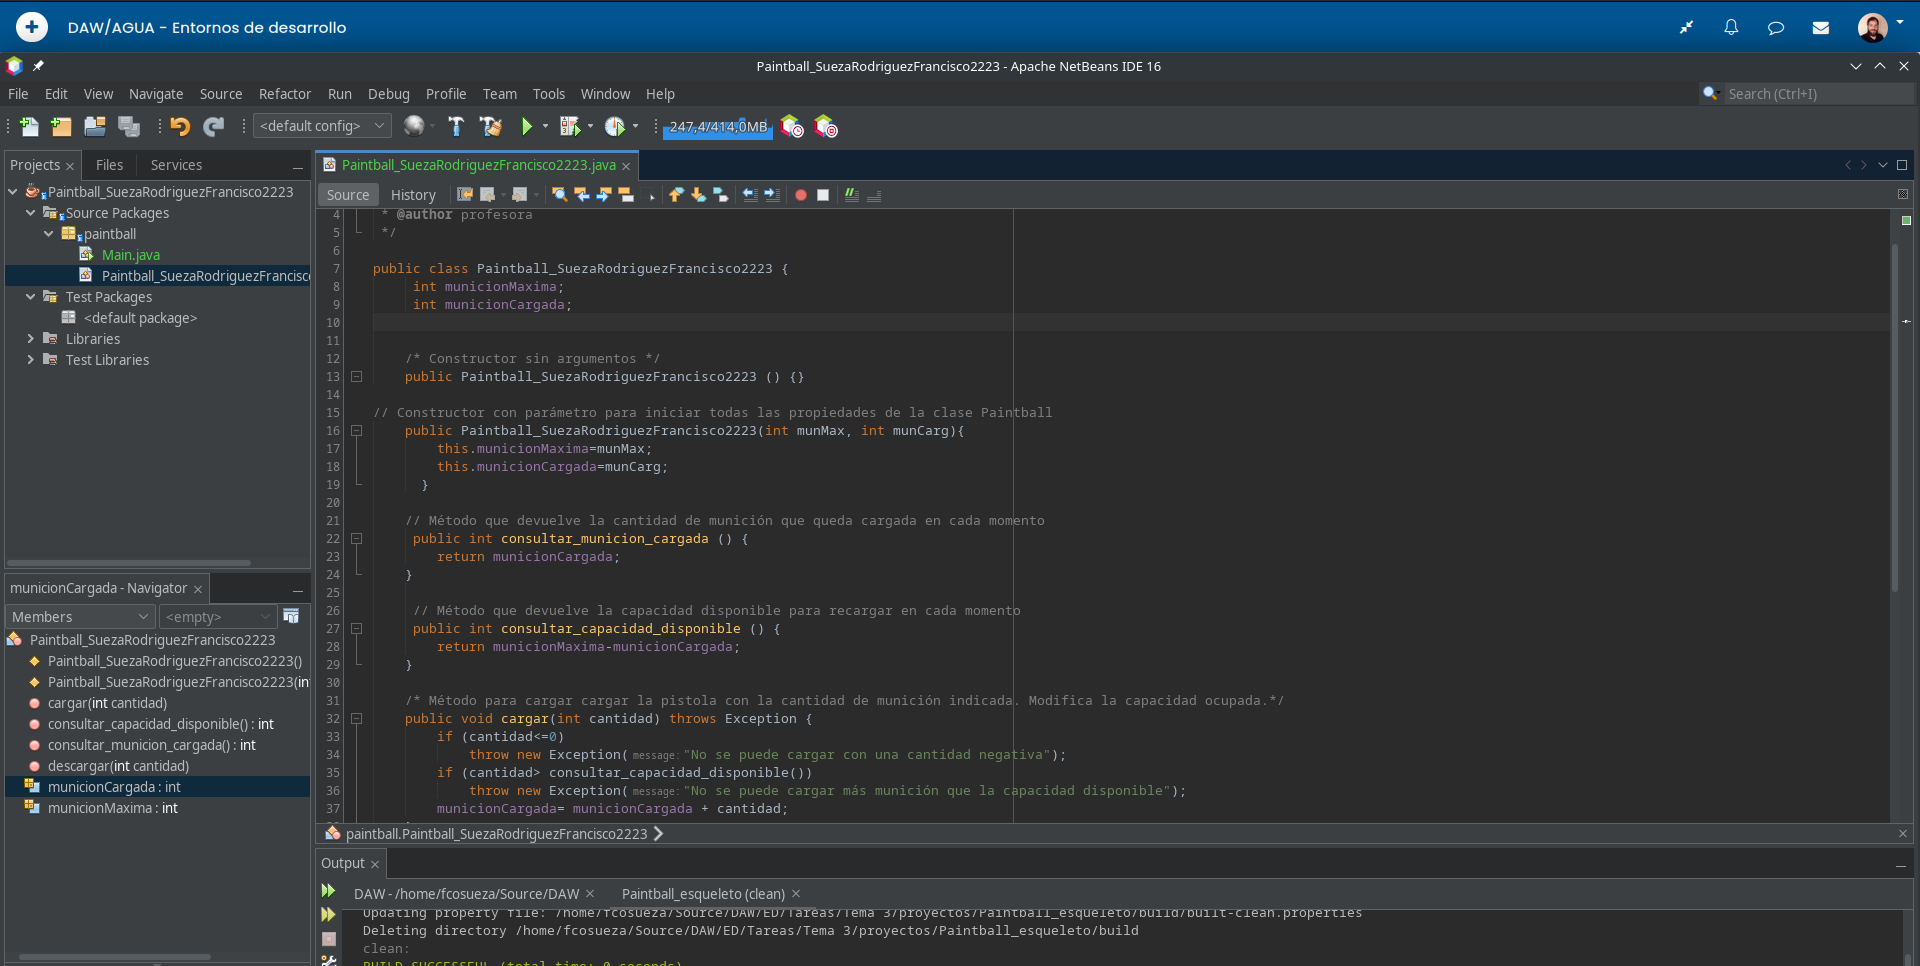
\includegraphics[scale=0.25]{cambio-nombre.png}
    \caption{Cambio de nombre del proyecto y la clase}
\end{figure}


\subsection{Actividad 2}

En este segundo punto hemos realizado la ejecución paso a paso del programa y se han realizado dos capturas mostrando el valor de la variable \textbf{municionCargada} tras la ejecución del método \textbf{miPaintball.descargar(10)} y \textbf{miPaintball.cargar(5)}.

Para ello, solo se ha tenido que modificar en la clase Main el valor asignación de la variable x, que estaba establecido en 12 pero se nos pide que probemos con una valor de 10 el método descargar. La otra variable no ha sido necesaria, ya que esta ya establecidad en 5, que es el valor que se nos pide.

Se han establecido 2 puntos de ruptura en la clase en main, en concreto en las líneas 32 y 39, justo después de la ejecución de los métodos pedidos, para poder inspeccionar la variable municionCargada. Se han elegido estas líneas porque la expresión \textbf{catch}, justo después de la ejecución de los métodos solo se evalúa si se lanza una excepción, por lo que si la ejecución es normal, no se detendrá en un breakpoint establecido en esta línea.

\begin{figure}[ht]
    \centering
    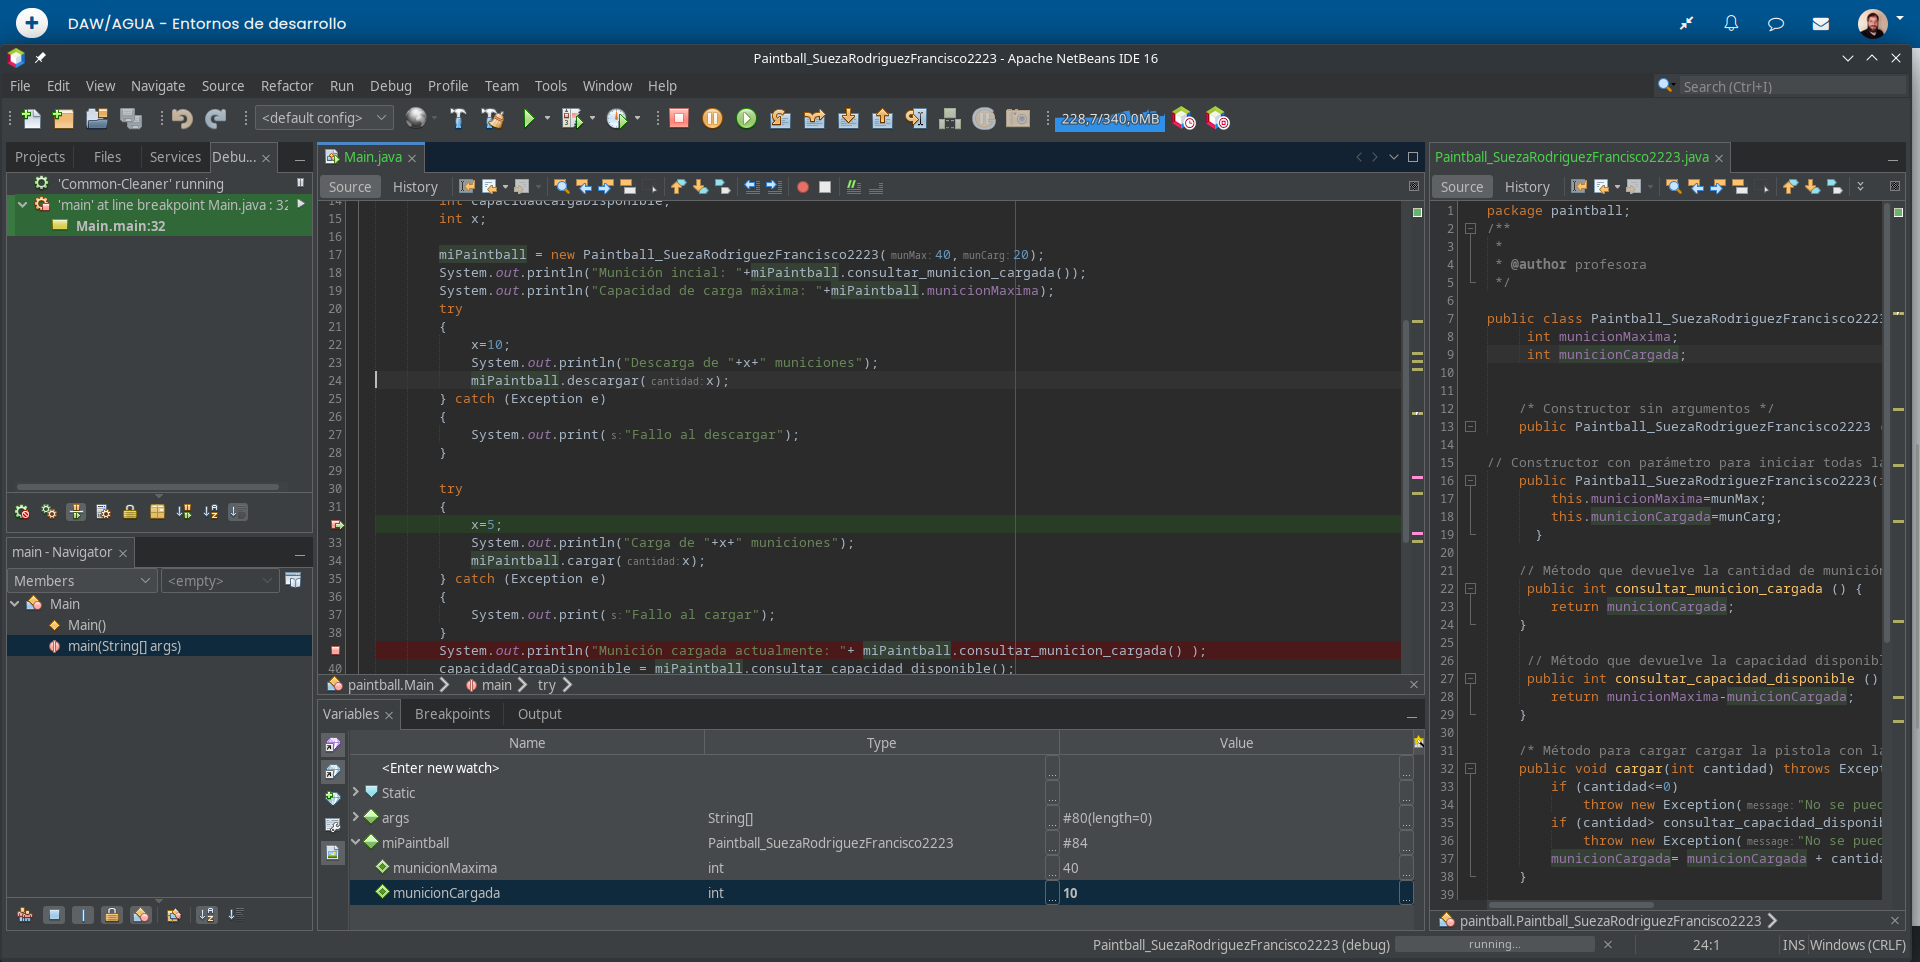
\includegraphics[scale=0.25]{watch-1.png}
    \caption{Captura de la variable municionCargada despues de miPaintball.descargar(10}
\end{figure}

Como vemos, el valor de la variable municionCargada despues de ejecutar el método miPaintball.descargar(10) es de \textbf{10}.

\begin{figure}[ht]
    \centering
    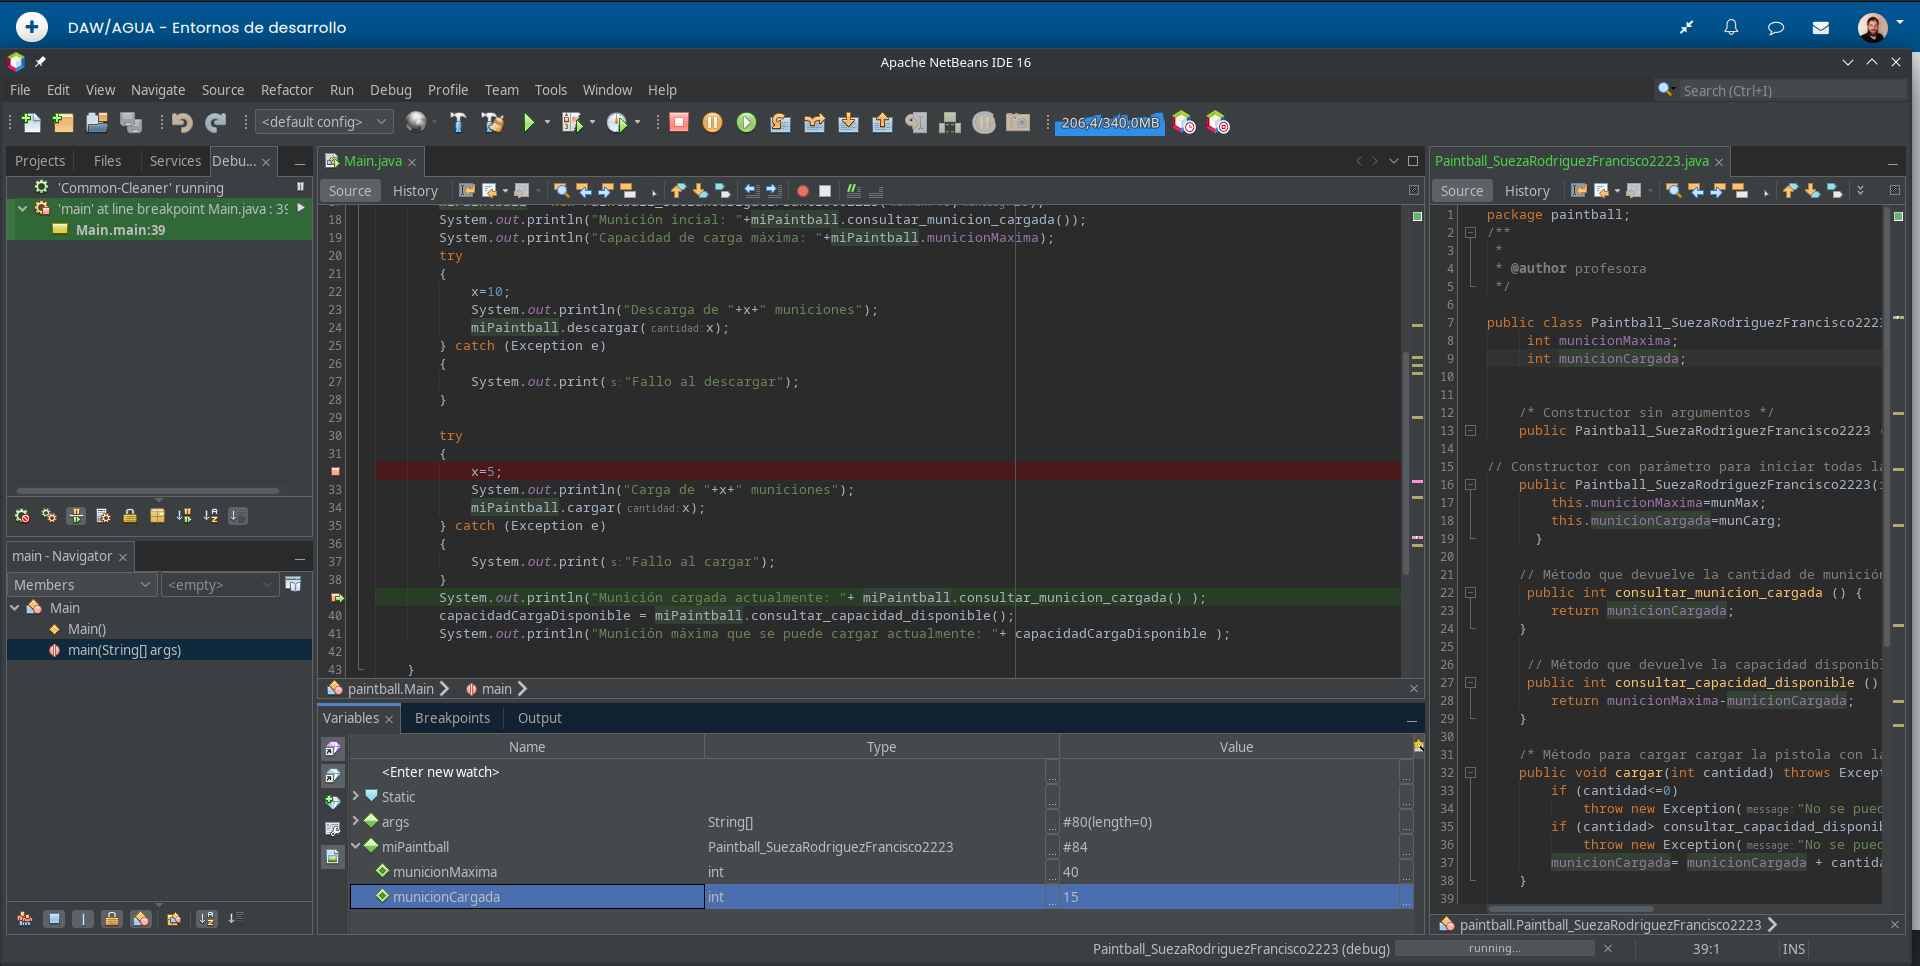
\includegraphics[scale=0.25]{watch-2.png}
    \caption{Captura de la variable municionCargada despues de miPaintball.cargar(5)}
\end{figure}

Después de la ejecución del método cargar, como vemos, el valor de la variable \textbf{municionCargada} es de \textbf{15}.

\subsection{Actividad 3}

A continuación se han diseñado los casos de prueba para el método \textbf{descargar} de la clase \textbf{Paintball}.

En este caso, vamos a testear los valores límite donde el \textbf{límite inferior} vendrá dado por el valor \textbf{0}, ya que no se pueden descargar 0 o menos municiones. El \textbf{límite superior} vendrá impuesto por la {cantidad de munición cargada}, ya que no se puede descargar más munición de la que tenemos cargada. Así, lo parámetros válidos estarían entre los valores \textbf{1} y \textbf{municionCargada}, incluidos los dos. Por lo tanto, los valores límite quedarían así:

\begin{itemize}
    \item \textbf{Valores límite validos}: 1, 2, (munición cargada - 1) y (munición cargada).
    \item \textbf{Valores límite no validos}: 0 y (munición cargada).
\end{itemize}

A continuación se pone el código de todos los test diseñados.

\begin{figure}[H]
    \begin{tcolorbox}[sharp corners, colback=yellow!30, colframe=white!20]
        \tiny
        \begin{verbatim}

public class Paintball_SuezaRodriguezFrancisco2223Test extends TestCase {
    public Paintball_SuezaRodriguezFrancisco2223Test(String testName) {
        super(testName);
    }

    @Override
    protected void setUp() throws Exception {
        super.setUp();
    }

    @Override
    protected void tearDown() throws Exception {
        super.tearDown();
    }
         \end{verbatim}
    \end{tcolorbox}
    \caption{Código Test Parte 1}
\end{figure}

\begin{figure}[H]
    \begin{tcolorbox}[sharp corners, colback=yellow!30, colframe=white!20]
        \tiny
        \begin{verbatim}
   /**
    * Tests para comprobar os valores límite sobre el método Descargar.
    */


    /**
    * Test para el método Descargar. En esta prueba se van intentar descargar 0
    * municiones, algo que no debería permitir el método.
    *
    * @result El metodo no debe permitir descargar 0 municiones, lanzando una excepcion.
    * @throws java.lang.Exception
    */

    @Test
    public void testDescargarCero() throws Exception {
        System.out.println("Test de prueba para intentar descargar 0 municiones");

        int municion = 0;
        int municionMaxima = 30;
        int municionCargada = 10;

        Paintball_SuezaRodriguezFrancisco2223 paintball =
        new Paintball_SuezaRodriguezFrancisco2223(municionMaxima, municionCargada);

        try {
            paintball.descargar(municion);
            fail("No se pueden descargar 0 municiones.");

        } catch(Exception e) {
            System.out.println(e);
            assertTrue(paintball.consultar_municion_cargada() == municionCargada);
        }
    }

   /**
    * Test para el método Descargar. En esta prueba se van intentar descargar 1
    * municiones, algo que debería permitir el metodo, restando esta cantidad
    * a la munición cargada
    *
    * @result El metodo debe permitir descargar 1 munición y restar 1 a municionCargada.
    * @throws java.lang.Exception
    */

    @Test
    public void testDescargarUno() throws Exception {
        System.out.println("Test de prueba para intentar descargar 1 municiones");

        int municion = 1;
        int municionMaxima = 30;
        int municionCargada = 10;

        Paintball_SuezaRodriguezFrancisco2223 paintball =
        new Paintball_SuezaRodriguezFrancisco2223(municionMaxima, municionCargada);

        try {
            paintball.descargar(municion);
            assertTrue(paintball.consultar_municion_cargada() == municionCargada - municion);

        } catch(Exception e) {
            fail("Se ha producido una excepción inesperada.");
        }
    }

   /**
    * Test para el método Descargar. En esta prueba se van intentar descargar 2
    * municiones, algo que debería permitir el metodo, restando esta cantidad
    * a la munición cargada
    *
    * @result El metodo debe permitir descargar 1 munición y restar 2 a la munición cargada.
    * @throws java.lang.Exception
    */

    @Test
    public void testDescargarDos() throws Exception {
        System.out.println("Test de prueba para intentar descargar 2 municiones");

        int municion = 2;
        int municionMaxima = 30;
        int municionCargada = 10;

        Paintball_SuezaRodriguezFrancisco2223 paintball =
        new Paintball_SuezaRodriguezFrancisco2223(municionMaxima, municionCargada);

        try {
            paintball.descargar(municion);
            assertTrue(paintball.consultar_municion_cargada() == municionCargada - municion);

        } catch(Exception e) {
            fail("Se ha producido una excepción inesperada.");
        }
    }

        \end{verbatim}
    \end{tcolorbox}
    \caption{Código Test Parte II}
\end{figure}

\begin{figure}[H]
    \begin{tcolorbox}[sharp corners, colback=yellow!30, colframe=white!20]
        \tiny
        \begin{verbatim}

   /**
    * Test para el método Descargar. En esta prueba se van intentar descargar (municionCargada - 1)
    * municiones, algo que debería permitir el metodo, restando esta cantidad a la munición cargada
    * quedando por tanto solo 1 munición en el cargador.
    *
    * @result El metodo debe permitir descargar (municionCargada - 1) municiones y restar esta cantidad
    *         dejando 1 municion en el cargador.
    * @throws java.lang.Exception
    */

    @Test
    public void testDescargarCargadaMenos() throws Exception {
        System.out.println("Test de prueba para intentar descargar (municionCargada - 1) municiones");

        int municionMaxima = 30;
        int municionCargada = 10;
        int municion = municionCargada - 1;

        Paintball_SuezaRodriguezFrancisco2223 paintball =
        new Paintball_SuezaRodriguezFrancisco2223(municionMaxima, municionCargada);

        try {
            paintball.descargar(municion);
            assertTrue(paintball.consultar_municion_cargada() == 1);

        } catch(Exception e) {
            fail("Se ha producido una excepción inesperada.");
        }
    }

   /**
    * Test para el método Descargar. En esta prueba se van intentar descargar (municionCargada)
    * municiones, algo que debería permitir el metodo, restando esta cantidad a la munición cargada
    * quedando por tanto solo 1 munición en el cargador.
    *
    * @result El metodo debe permitir descargar (municionCargada) municiones y restar esta cantidad
    *         dejando 0 municiones en el cargador.
    * @throws java.lang.Exception
    */

    @Test
    public void testDescargarCargada() throws Exception {
        System.out.println("Test de prueba para intentar descargar \"municionCargada\" municiones");

        int municionMaxima = 30;
        int municionCargada = 10;
        int municion = municionCargada;

        Paintball_SuezaRodriguezFrancisco2223 paintball =
        new Paintball_SuezaRodriguezFrancisco2223(municionMaxima, municionCargada);

        try {
            paintball.descargar(municion);
            assertTrue(paintball.consultar_municion_cargada() == 0);

        } catch(Exception e) {
            fail("Se ha producido una excepción inesperada.");
        }
    }

   /**
    * Test para el método Descargar. En esta prueba se van intentar descargar (municionCargada + 1)
    * municiones, algo que no debería permitir, lanzando una excepción.
    *
    * @result El metodo no debe permitir descargar más munición de la que hay, lanzando un excepción..
    * @throws java.lang.Exception
    */

    @Test
    public void testDescargarCargadaMas() throws Exception {
        System.out.println("Test de prueba para intentar descargar (municionCargada + 1) municiones");

        int municionMaxima = 30;
        int municionCargada = 10;
        int municion = municionCargada + 1;

        Paintball_SuezaRodriguezFrancisco2223 paintball =
        new Paintball_SuezaRodriguezFrancisco2223(municionMaxima, municionCargada);

        try {
            paintball.descargar(municion);
            fail("No se pueden descargar más municiones de las que hay cargadas.");

        } catch(Exception e) {
            System.out.println(e);
            assertTrue(paintball.consultar_municion_cargada() == municionCargada);
        }
    }

        \end{verbatim}
    \end{tcolorbox}
    \caption{Código Test Parte III}
\end{figure}

\subsection{Actividad 4}
Una vez realizadas las pruebas para los valores límites, vamos a realizar pruebas para los valores no válidos en general. En este caso, teniendo en cuenta las clases de equivalencia que podríamos tener, vamos a crear 2 test, para probar los valores \textbf{-100} y (munición cargada + 100). Ya en el ejercicio anterior hemos probado algunos valores no válidos, pero estos pertenecían a los valores límite, como era el caso de 0 y (munición cargada + 1).

En la siguiente figura podemos ver el código de estos test.

\begin{figure}[H]
    \begin{tcolorbox}[sharp corners, colback=yellow!30, colframe=white!20]
        \tiny
        \begin{verbatim}
/**
 * Test para probar valores no validos fuera de los valores límite.
 */

/**
 * Test para el método Descargar.  Se va a probar un valor no valido negativo.
 *
 * @result El metodo no debe permitir descargar un número negativo de munición.
 * @throws java.lang.Exception
 */

@Test
public void testNoValidoNegativo() throws Exception {
    System.out.println("Test de prueba para intentar descargar -100 municiones.");

    int municionMaxima = 30;
    int municionCargada = 10;
    int municion = -500;

    Paintball_SuezaRodriguezFrancisco2223 paintball =
        new Paintball_SuezaRodriguezFrancisco2223(municionMaxima, municionCargada);

    try {
        paintball.descargar(municion);
        fail("No se pueden descargar un número negativo de municiones.");

    } catch(Exception e) {
        System.out.println(e);
        assertTrue(paintball.consultar_municion_cargada() == municionCargada);
    }
}

/**
 * Test para el método Descargar.  Se va a probar un valor no valido positivo, que sera
 * muy superior a la cantidad de munición cargada.
 *
 * @result El metodo no debe permitir descargar un número positivo no valido.
 * @throws java.lang.Exception
 */

@Test
public void testNoValidoPositivo() throws Exception {
    System.out.println("Test para descargar (municion cargada + 500) municiones");

    int municionMaxima = 30;
    int municionCargada = 10;
    int municion = municionCargada + 500;

    Paintball_SuezaRodriguezFrancisco2223 paintball =
        new Paintball_SuezaRodriguezFrancisco2223(municionMaxima, municionCargada);

    try {
        paintball.descargar(municion);
        fail("No se pueden descargar más munición de la que hay cargada");

    } catch(Exception e) {
        System.out.println(e);
        assertTrue(paintball.consultar_municion_cargada() == municionCargada);
    }
}
        \end{verbatim}
    \end{tcolorbox}
    \caption{Documento SGML simple}
\end{figure}

\subsection{Actividad 5}
Por último, se han ejecutado los test de prueba. En este caso se han pasado todos los test salvo uno, como podemos ver en la siguiente captura de pantalla.

\begin{figure}[ht]
    \centering
    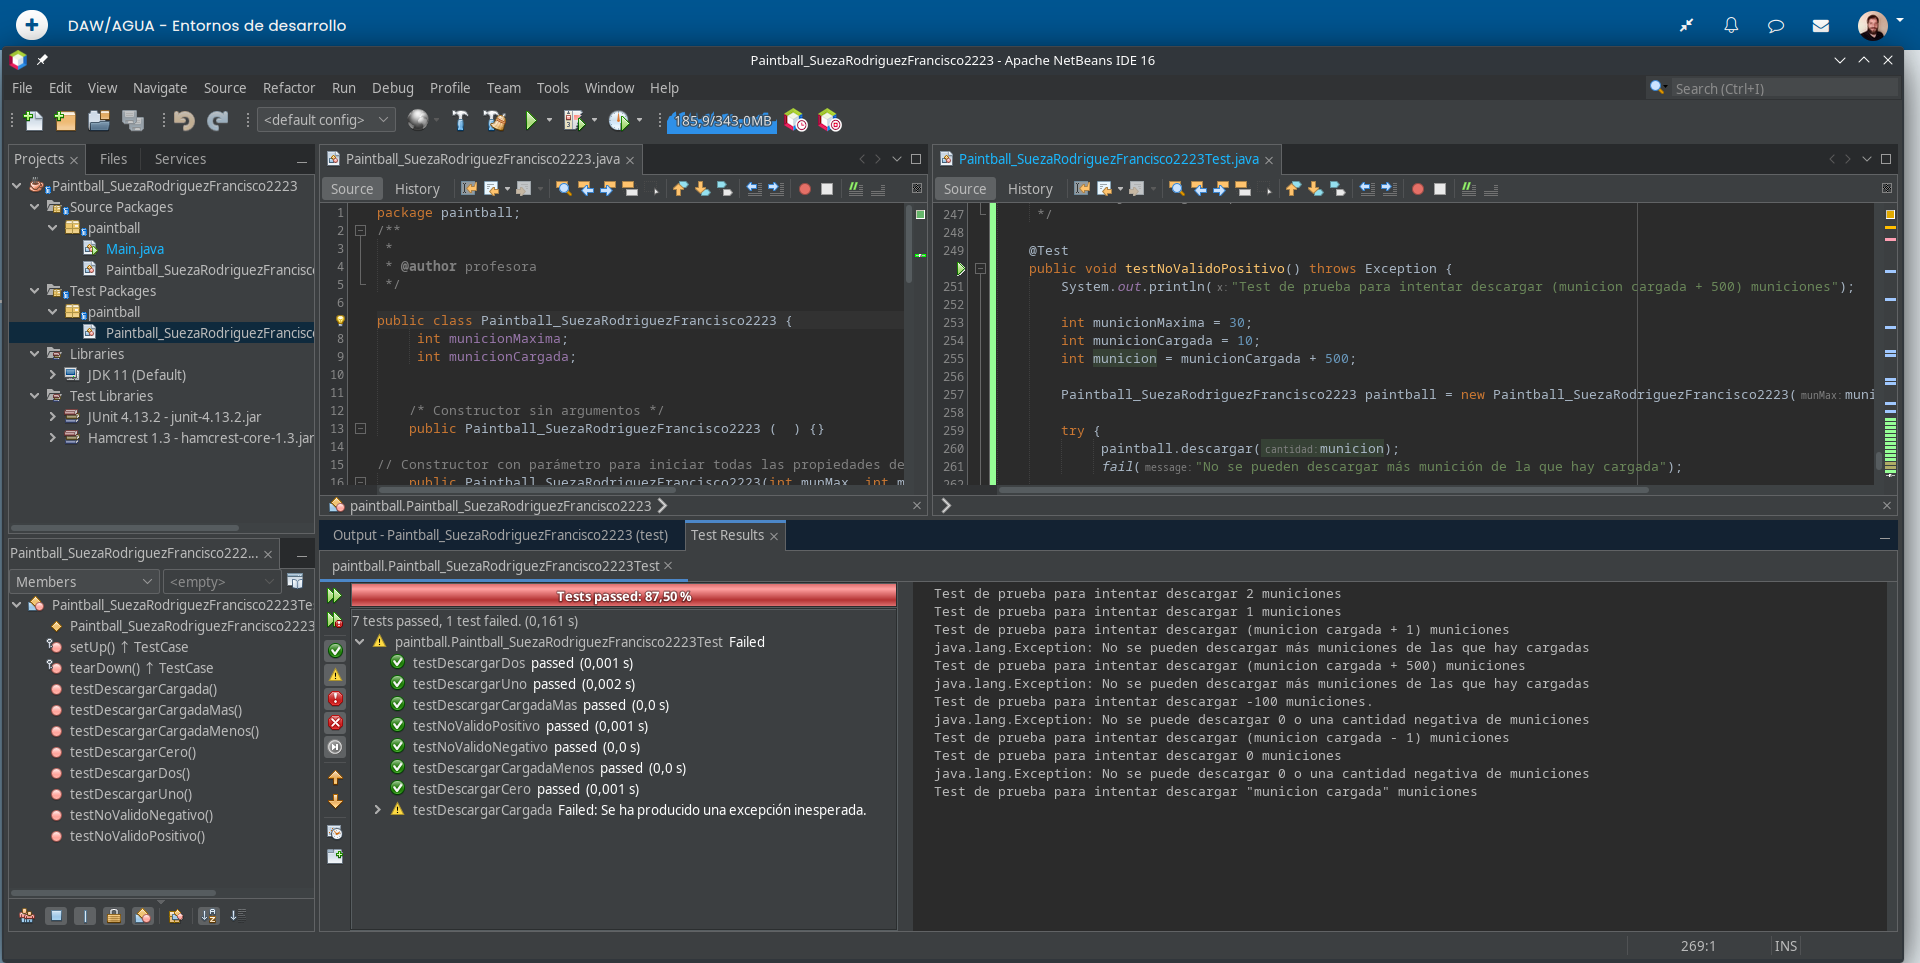
\includegraphics[scale=0.25]{ejecucion-test.png}
    \caption{Ejecución de los test}
\end{figure}

Como podemos ver, el test que ha fallado ha sido \textbf{descargarCargada}. Este test trataba de descargar la misma cantidad de munición que había cargada, lo que entraba dentro de la categoría de los \textbf{valores límite válidos}, por lo que el método debería permitir llevar a cabo esta acción. Ya que este test ha resultado fallido, mientras que el resto se han pasado sin problema, podemos pensar que hay algún error en la parte que comprueba la cantidad de munición que se quiere descargar sobre la cargada.

Si nos vamos al código del método en la clase Paintball, el error se ve rápidamente, y es que hay una sentencia \textbf{if...else}, donde se comprueba si la munición que se quiere descargar es mayor que la munición cargada, el problema es que la condición esta escrita así \textit{cantidad>=municionCargada}, por que no solo no se permite descargar la munición que supera a la cantidad cargada, sino que que tampoco permite descargar una cantidad igual a esta.

Para solucionarlo, bastaría con cambiar el operador con el que se realiza la comprobación, quedando esta condición así \textit{cantidad>municionCargada}.

% Bibliography
\newpage
\bibliography{citas}
\bibliographystyle{unsrt}

\end{document}